% vim: set tw=78 sts=2 sw=2 ts=8 aw et ai:
\documentclass{workshop}

% Comentează liniile de mai jos în cazul în care nu există cod de inclus.
\usepackage{code/highlight}
\usepackage{color}        % dacă e folosit highlight
\usepackage{alltt}        % dacă e folosit highlight
\usepackage{amsmath}

\title[Session 3]{Session 3}
\subtitle{Introduction to Kernel Space and API}
\author{Daniel Băluță, Alex Juncu, Irina Preșa}
\date{03 July 2013}

\begin{document}

% Arătăm numărul frame-ului
\setbeamertemplate{footline}[frame number]

\frame{\titlepage}

% NB: Secțiunile nu sunt marcate vizual, ci doar apar în cuprins
\section{In the kernel world}

\begin{frame}{Execution Contexts}
  \begin{itemize}
    \item \textbf{Interrupt context}
    \item \textbf{Process context}
    \begin{itemize}
      \item User space
      \item Kernel space
    \end{itemize}
  \end{itemize}
\end{frame}


\begin{frame}{User space vs Kernel space}
  \begin{figure}
    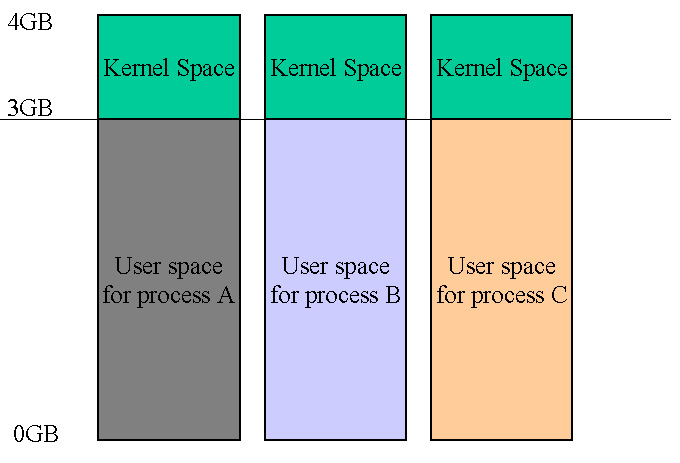
\includegraphics[scale=0.4]{img/user-kernel-space.jpg}
  \end{figure}
\end{frame}

\begin{frame}{System calls}
  \begin{itemize}
    \item \emph{syscall()}
    \item CPU moves to Ring 0 access level
    \item Access to all Virtual Memory
  \end{itemize}
\end{frame}



\section{Kernel API}
\begin{frame}{Kernel API}
\begin{itemize}
\item printk, classical string operations
\item kmalloc/kfree
\item lists: doubly linked list API
\item locking
\end{itemize}
\end{frame}

\begin{frame}{Simple dynamic memory... ish...}
  \begin{itemize}
    \item \emph{kmalloc}
    \begin{itemize}
     \item GFP\_KERNEL/ATOMIC
     \end{itemize}
    \item \emph{kfree}
    \begin{itemize}
     \item always, always, ALWAYS free unused memory
     \item ...but not twice for the same memory
     \end{itemize}
  \end{itemize}
\end{frame}



\begin{frame}{Lists}
  \begin{itemize}

    \item LIST_HEAD(name)
    \item INIT_LIST_HEAD(struct list_head *list)
    \item list_add(struct list_head *new, struct list_head *head)
    \item list_del(struct list_head *entry)
    \item list_entry(ptr, type, member)
    \item list_for_each(pos, head)
    \item list_for_each_safe(pos, n, head)
  \end{itemize}
\end{frame}

\begin{frame}{Kernel API - Lists Example}
\input{code/list}
\end{frame}

\begin{frame}{Kernel API - Lists Example}
  \begin{figure}
    \includegraphics[scale=0.2]{img/list.png}
  \end{figure}
\end{frame}


\begin{frame}{Synconization and locking}
  \begin{itemize}
    \item spinlocks
    \item semaphores
    \item atomic variables
  \end{itemize}
\end{frame}


\begin{frame}{Spinlocks}
  \begin{itemize}
    \item DEFINE_SPINLOCK(lock1);
    \item spinlock_t lock2; spin_lock_init(\&lock2);
    \item spin_lock(\&lock1);
    \item spin_unlock(\&lock1);
  \end{itemize}
\end{frame}








\section{Keywords}
\begin{frame}{Keywords}
  \begin{columns}
    \begin{column}[l]{0.5\textwidth}
      \begin{itemize}
        \item process context
        \item interrupt context
        \item user space
        \item kernel space
        \item syscalls
      \end{itemize}
    \end{column}
    \begin{column}[l]{0.5\textwidth}
      \begin{itemize}
        \item kernel API
        \item kmalloc
        \item kfree
        \item lists
        \item locking
      \end{itemize}
    \end{column}
  \end{columns}
\end{frame}

\section{Resources}
\begin{frame}{Resources}
  \begin{itemize}
  \item \href{http://elf.cs.pub.ro/so2/wiki/}{SO2 Course}
  \item \href{http://www.ibm.com/developerworks/linux/library/l-proc/index.html}{Access procfs}
  \item \href{http://articles.manugarg.com/systemcallinlinux2_6.html}{System Calls}
  \item \href{http://www.kernel.org/pub/linux/kernel/people/rusty/kernel-locking/c214.html}{Kernel Locking}
  \end{itemize}
\end{frame}

\section{Questions}

\end{document}
